%-------------------------------------------------
% FileName: chapt-2.tex
% Author: Safin (zhaoqid@zsc.edu.cn)
% Version: 0.1
% Date: 2020-05-12
% Description: 第2章
% Others: 
% History: origin
%------------------------------------------------- 

% 断页
% \clearpage
\chapter{RISC-V处理器介绍}

\section{RISC-V处理器指令集}

\subsection{指令集格式}

RISC-V 基础指令集(Base ISA)作为 RISC-V 架构的核心,为处理器提供了基本的指令集框架。如表\ref{tab:riscv_instruction_formats}和图\ref{fig:riscv_instruction_formats}所示,RV32I 包含了六种基本指令类型:
\begin{enumerate}[label={\arabic*)},itemsep=0pt, parsep=0pt]
	\item \textbf{R型}:两个操作数来自寄存器,用于寄存器间操作;
	\item \textbf{I型}:两个操作数来自立即数和寄存器,用于实现立即数和取数操作;
	\item \textbf{S型}:两个操作数来自寄存器,一个操作数来自立即数,用于实现访存操作;
	\item \textbf{B型}:两个操作数来自寄存器,一个操作数来自立即数,用于实现条件分支操作;
	\item \textbf{U型}:一个操作数来自立即数,用于实现长立即数操作;
	\item \textbf{J型}:一个操作数来自立即数,用于实现无条件跳转操作。
\end{enumerate}

从指令格式就可以看出RISC-V指令集最大的优点——精简。首先,指令的长度都为32位,同一种类型的指令格式单一,大幅度减小了译码器的开销以及实现难度。其次,R型指令提供了三个寄存器,这对于需要三个操作数的指令不需要额外的访存,避免了访存带来的开销。然后,寄存器的编码都在指令的固定位置(rs1和rs2),在译码之前就可以先读取寄存器的值读。最后,立即数的符号位被编码至指令的最高位,所以,立即数的符号扩展操作可以与译码操作并行处理。

%绘制RV32I指令结构
\begin{figure}[htbp]
	\centering % 使图像居中
	\begin{adjustbox}{width=0.9\textwidth} % 设置图像宽度为页面宽度的 0.9 倍
		% 这里是你的 bytefield 表格代码
		\begin{bytefield}[bitwidth=1.2em, boxformatting={\centering}, endianness=big]{32}
			% R-type (Register-Register)
			\bitheader{31,25,24,20,19,15,14,12,11,7,6,0} \\ % 显示边界条件的坐标
			\bitbox{7}{funct7} & \bitbox{5}{rs2} & \bitbox{5}{rs1} & \bitbox{3}{funct3} & \bitbox{5}{rd} & \bitbox{7}{opcode} \\
			\wordbox[]{1}{R-type (Register-Register)} \\

			% I-type (Immediate)
			\bitheader{31,20,19,15,14,12,11,7,6,0} \\
			\bitbox{12}{imm[11:0]} & \bitbox{5}{rs1} & \bitbox{3}{funct3} & \bitbox{5}{rd} & \bitbox{7}{opcode} \\
			\wordbox[]{1}{I-type (Immediate)} \\

			% S-type (Store)
			\bitheader{31,25,24,20,19,15,14,12,11,7,6,0} \\
			\bitbox{7}{imm[11:5]} & \bitbox{5}{rs2} & \bitbox{5}{rs1} & \bitbox{3}{funct3} & \bitbox{5}{imm[4:0]} & \bitbox{7}{opcode} \\
			\wordbox[]{1}{S-type (Store)} \\

			% B-type (Branch)
			\bitheader{31,25,24,20,19,15,14,12,11,7,6,0} \\
			\bitbox{7}{imm[12|10:5]} & \bitbox{5}{rs2} & \bitbox{5}{rs1} & \bitbox{3}{funct3} & \bitbox{5}{imm[4:1|11]} & \bitbox{7}{opcode} \\
			\wordbox[]{1}{B-type (Branch)} \\

			% U-type (Upper Immediate)
			\bitheader{31,12,11,7,6,0} \\
			\bitbox{20}{imm[31:12]} & \bitbox{5}{rd} & \bitbox{7}{opcode} \\
			\wordbox[]{1}{U-type (Upper Immediate)} \\

			% J-type (Jump)
			\bitheader{31,12,11,7,6,0} \\
			\bitbox{20}{imm[20|10:1|11|19:12]} & \bitbox{5}{rd} & \bitbox{7}{opcode} \\
			\wordbox[]{1}{J-type (Jump)} \\
		\end{bytefield}
	\end{adjustbox}
	\caption{RV32I 指令集格式} % 添加题注
	\label{fig:riscv_instruction_formats}
\end{figure}

%绘制指令类型介绍
\begin{table}[htbp]
	\centering
	\caption{RISC-V 指令格式介绍}
	\begin{tabularx}{\textwidth}{>{\centering\arraybackslash}X >{\centering\arraybackslash}X >{\centering\arraybackslash}X}
		\toprule
		\textbf{类型}   & \textbf{用途} & \textbf{示例指令}              \\
		\midrule
		R型(寄存器-寄存器操作) & 算术和逻辑运算     & \texttt{add x1, x2, x3}    \\
		% \cmidrule{1-3}
		I型(立即数操作)     & 加载、立即数操作和跳转 & \texttt{addi x1, x2, 10}   \\
		% \cmidrule{1-3}
		S型(存储操作)      & 数据从寄存器存储到内存 & \texttt{sw x1, 12(x2)}     \\
		% \cmidrule{1-3}
		B型(条件分支)      & 条件分支跳转      & \texttt{beq x1, x2, label} \\
		% \cmidrule{1-3}
		U型(高位立即数操作)   & 加载高位立即数     & \texttt{lui x1, 0x12345}   \\
		% \cmidrule{1-3}
		J型(无条件跳转)     & 函数调用或长跳转    & \texttt{jal x1, label}     \\
		\bottomrule
	\end{tabularx}
	\label{tab:riscv_instruction_formats}
\end{table}

\subsection{通用寄存器}

如图\ref{tab:riscv_instruction_register}表示,RISC-V有32个寄存器,特殊的是,x0寄存器硬连线为0,可替代约15\%的指令操作,而X86需要显式XOR清零。为了提升处理器的性能,数据应该尽量存储在寄存器中,但是频繁的恢复和保存寄存器需要不断地访问内存,会带来不小的开销。为了避免这种情况,RISC-V的处理方案是设置临时寄存器(t0-6)和保存寄存器(s0-11)。临时寄存器的值不需要保存至内存,而保存寄存器的值需要保存至内存。

相比X86的16个寄存器,RISC-V架构的寄存器数量多一倍,适当地提升寄存器的数量,处理器可以充分地调度更多的寄存器,以至于加快程序编译和运行的速度。但是,寄存器并不是越多越好,由于其制造工艺和其特殊性导致了寄存器的成本昂贵,所以更多的寄存器会导致更高的成本和硬件复杂度,指令集也需要更多的比特位来对寄存器进行编码,一定程度上压缩了其余字段的编码空间,会提升编码和译码的复杂度。

%绘制寄存器表格
\begin{table}[htbp]
	\centering
	\caption{RISC-V 寄存器介绍}
	\begin{tabularx}{\textwidth}{>{\centering\arraybackslash}X >{\centering\arraybackslash}X >{\centering\arraybackslash}X}
		\toprule
		\textbf{寄存器} & \textbf{名称} & \textbf{功能} \\
		\midrule
		x0           & zero        & 始终为0        \\
		x1           & ra          & 返回地址        \\
		x2           & sp          & 栈指针         \\
		x3           & gp          & 全局指针        \\
		x4           & tp          & 线程指针        \\
		x5           & t0          & 临时寄存器/链接寄存器 \\
		x6-7         & t1-2        & 临时寄存器       \\
		x8           & fp / s0     & 帧指针/保存寄存器   \\
		x9           & s1          & 保存寄存器       \\
		x10-11       & a0-1        & 函数参数/返回值    \\
		x12-17       & a2-7        & 函数参数        \\
		x18-27       & s2-11       & 保存寄存器       \\
		x28-31       & t3-6        & 临时寄存器       \\
		\bottomrule
	\end{tabularx}
	\label{tab:riscv_instruction_register}
\end{table}

\subsection{指令集扩展}

RISC-V 指令集的另一个显著特点是模块化设计。RV32I 作为基础 ISA,虽然只定义了47条指令,但是足以支持运行基本的软件,其稳定性为开发者提供了可靠的指令集基础。模块化设计允许开发者根据具体需求选择特定的扩展,例如:
\begin{enumerate}[label={\arabic*)},itemsep=0pt, parsep=0pt]
	\item \textbf{RV32M}:支持乘除法扩展,从基本指令集分离出来的一个单独标准,需要设计对应的乘除法单元,适用于嵌入式系统、低功耗微控制器、高效处理整数运算的场景;
	\item \textbf{RV32A}:支持原子指令扩展,对共享内存的数据进行操作的一种方式,能够保证多线程并发执行的一致性,适用于多核处理器、操作系统内核、实时系统的场景;
	\item \textbf{RV32F}:支持单精度浮点扩展,新增了浮点寄存器,支持单精度浮点的传输、比较、转换、分类,适用于图形处理、传感器数据处理、轻量级机器学习推理的场景;
	\item \textbf{RV32D}:支持双精度浮点扩展,将浮点寄存器扩展至64位,新增了支持双精度浮点数相关的运算,适用于科学计算、高精度工程仿真、复杂模型训练的场景;
	\item \textbf{RV32V}:支持向量扩展,用于数据并行执行功能,该扩展引入了新的向量寄存器和操作指令,该扩展使RISC-V对于数据处理产生了质的提升,同时也保持了指令的简洁度。
\end{enumerate}

这种灵活的扩展机制使得 RISC-V 能够适应从嵌入式系统到高性能计算的多样化应用场景,如:物联网设备只需 RV32M + RV32F,而科学计算需要 RV32F + RV32D。这种设计理念为芯片设计者、软件开发者和终端用户带来了多方面的好处。

\subsection{特权指令集}

RISC-V 特权指令集(Privileged Instruction Set)定义了处理器在系统级操作中的行为规范,包括中断处理、内存管理、特权模式切换等核心功能。它是操作系统、监控程序(Hypervisor)和底层固件开发的基础。如\ref{tab:riscv_csr_state}所示,RISC-V目前有以下4种特权模式:U模式(User,用户模式),S模式(Supervisor,管理模式),H模式(Hypervisor,监视模式),M模式(Machine,M模式)。RISC-V通过CSR(控制状态寄存器)来更改权限模式。

%绘制CSR表格
\begin{table}[htbp]
	\centering
	\caption{RISC-V 特权模式}
	\begin{tabularx}{\textwidth}{>{\centering\arraybackslash}X >{\centering\arraybackslash}X >{\centering\arraybackslash}X}
		\toprule
		\textbf{等级} & \textbf{CSR编码} & \textbf{模式} \\
		\midrule
		0           & 00             & U           \\
		1           & 01             & S           \\
		2           & 10             & H           \\
		3           & 11             & M           \\
		\bottomrule
	\end{tabularx}
	\label{tab:riscv_csr_state}
\end{table}

\begin{enumerate}[label={\arabic*)},itemsep=0pt, parsep=0pt]
	\item \textbf{U模式}:用户模式是最低级的特权模式,只支持最低级别的权限操作,运行应用程序,禁止直接访问硬件或特权指令;
	\item \textbf{S模式}:管理模式拥有次高特权级,可以操作计算机中的敏感资源,用于管理虚拟内存、进程调度和系统调用;
	\item \textbf{H模式}:监视模式拥有比S模式更高的特权级,可以用于管理跨机器的资源,如管理多个虚拟机;
	\item \textbf{M模式}:机器模式拥有最高的特权级,可以执行任何机器操作,能访问所有物理资源(如定时器、中断控制器、PMP)的模式。
\end{enumerate}


\section{RISC-V汇编}
由于C程序无法直接运行在计算机上,所以需要将源代码翻译成为机器语言,才能在计算机上运行,该过程涉及编译、汇编、链接、载入,图\ref{fig:compile}展示了整个翻译过程。

\begin{figure}[htbp]
	\centering
	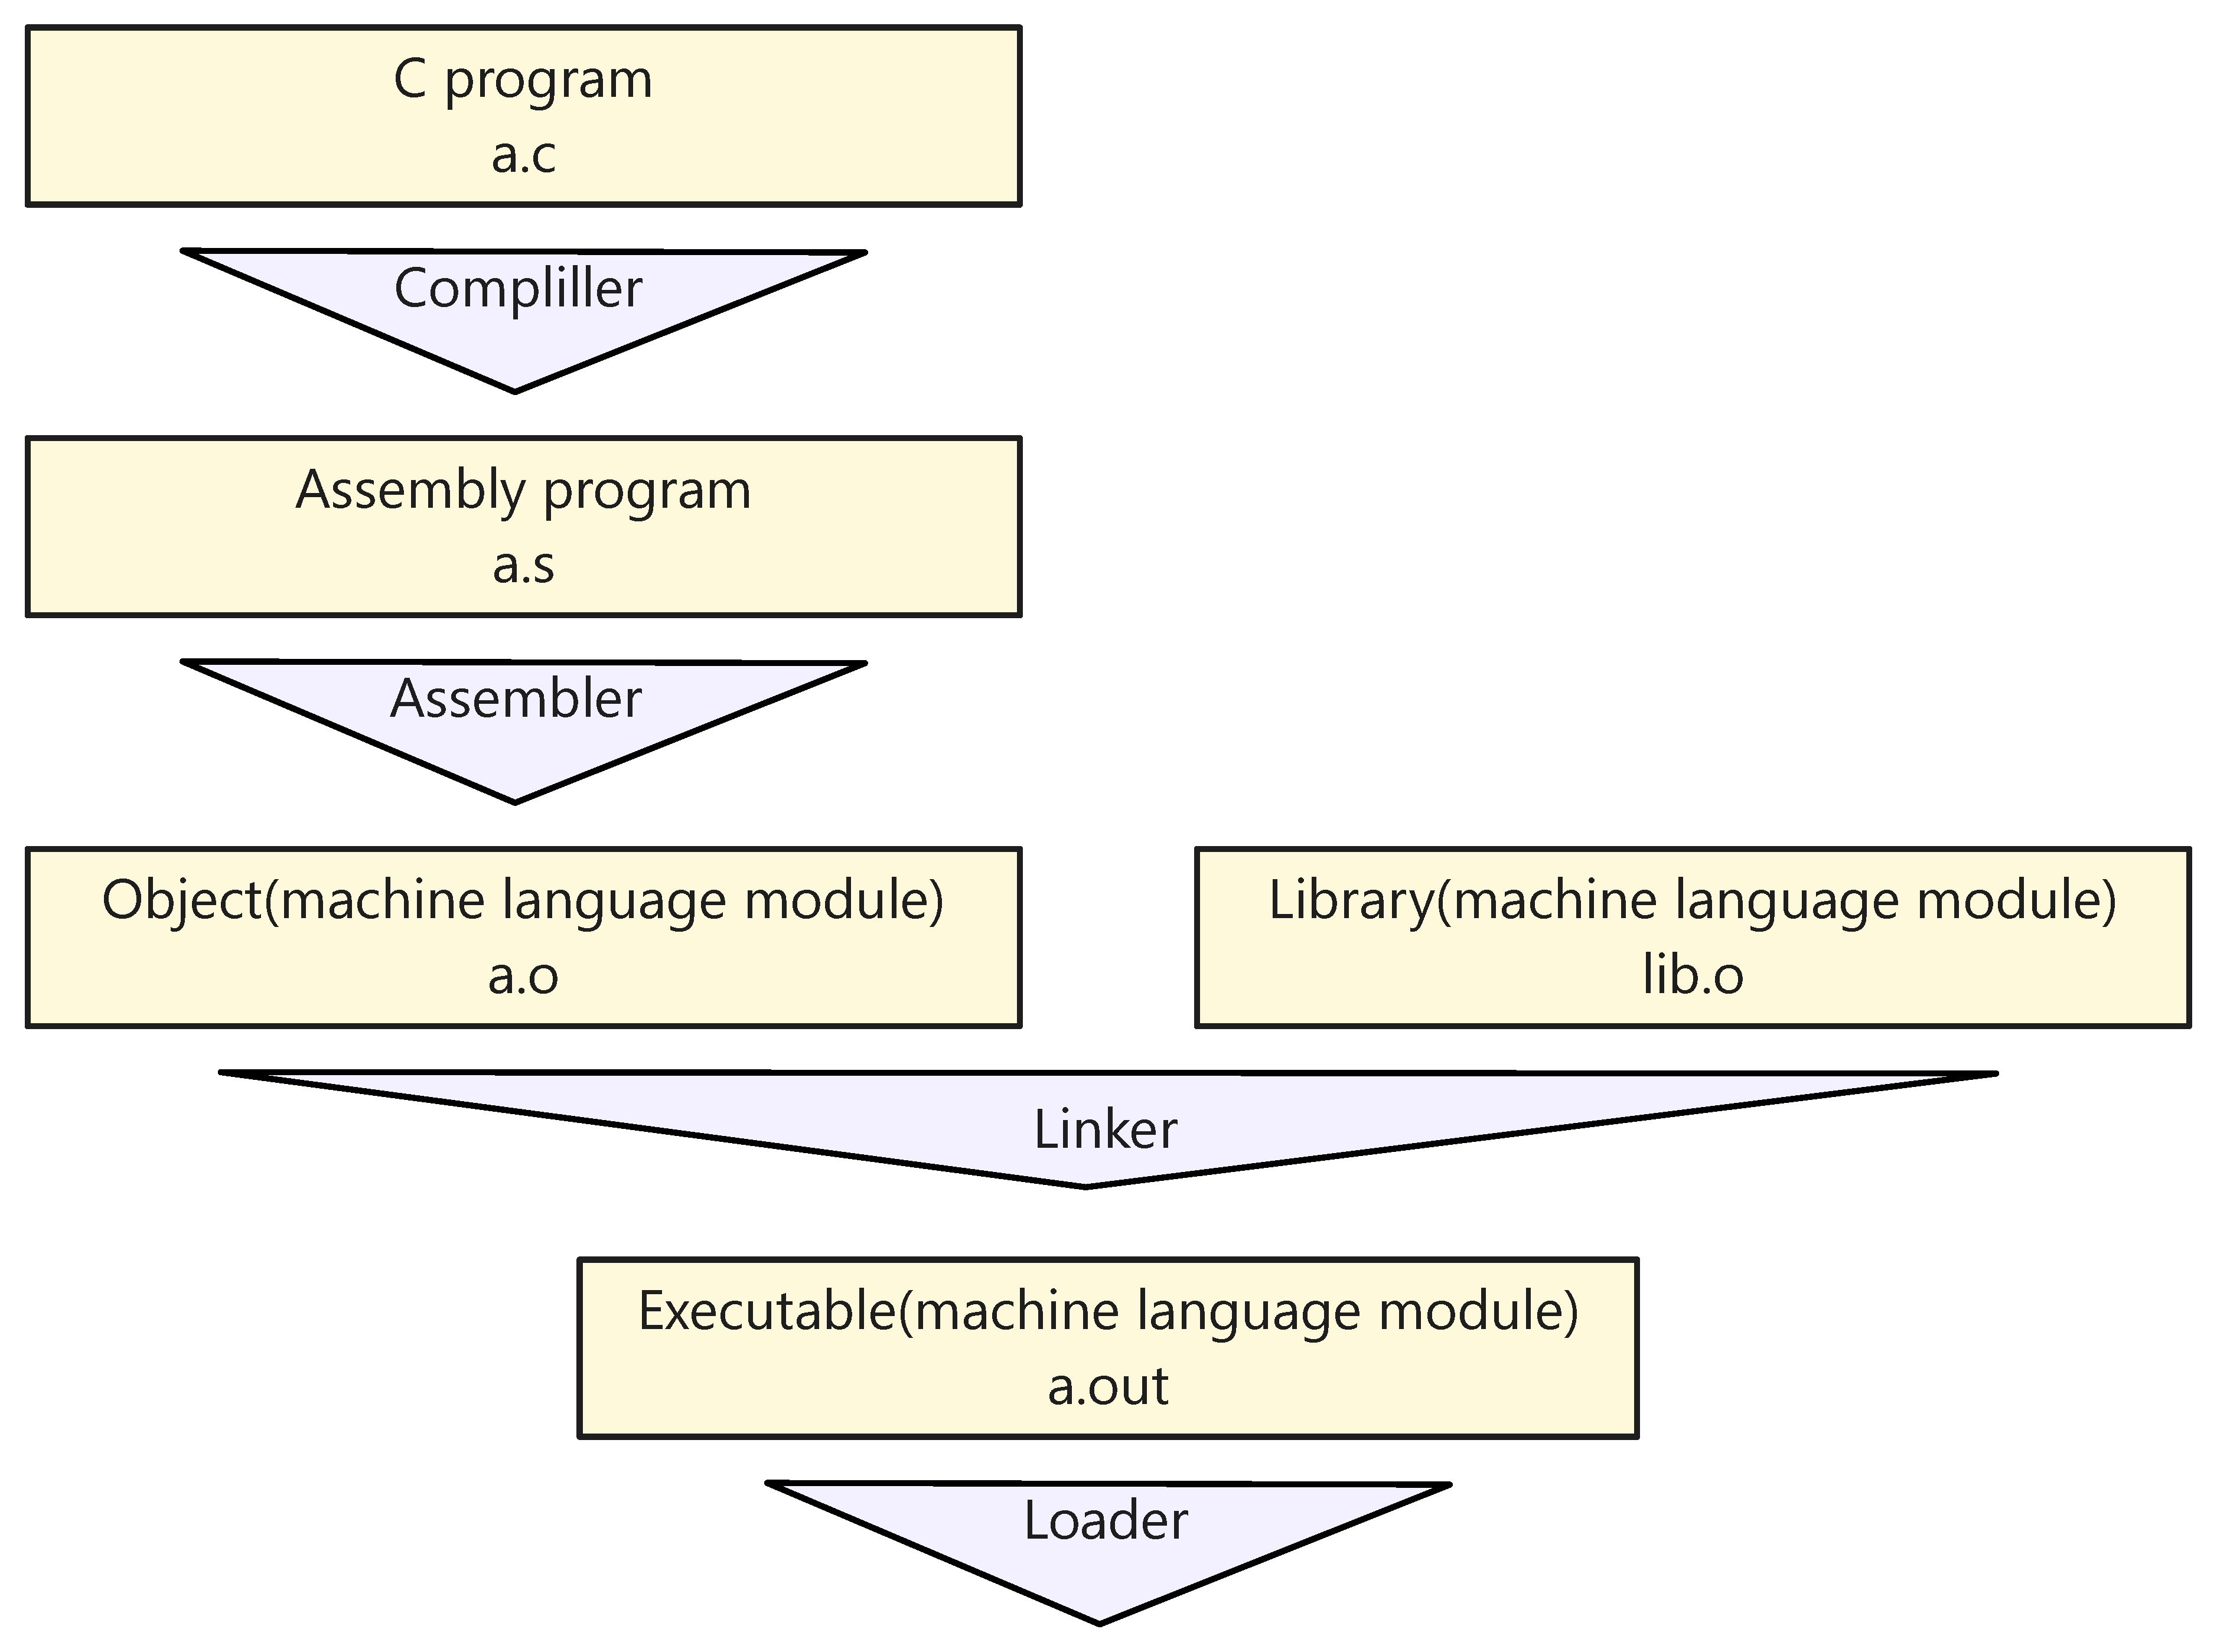
\includegraphics[width=0.8\textwidth]{image/compile.pdf}
	\caption{C源代码的翻译过程}
	\label{fig:compile}
\end{figure}

\subsection{编译器}
编译器是一类程序,用于将高级语言转换为机器语言指令集。如表\ref{tab:riscv_abi_state}所示,RISC-V编译器支持多种ABI(应用程序二进制接口),具体使用的接口取决于处理器所支持的扩展(例如F、D扩展)。其中,ilp32表示在C语言中int、long和pointer均为32位。后缀则表示浮点参数的传递方式:ilp32表示浮点参数通过整数寄存器传递;ilp32f表示单精度浮点参数通过浮点寄存器传递;ilp32d表示双精度浮点参数通过浮点寄存器传递。

因此,编译RV32I指令集的代码时,ABI选项必须为ilp32(GCC参数为:-march=rv32i -mabi=ilp32)。然而,在RISC-V的约定中,浮点指令的函数调用不一定需要使用浮点寄存器。这意味着,当编译支持RV32IFD指令集的代码时,ABI选项可以是ilp32、ilp32f或ilp32d中的任意一种。这种灵活性使得开发者能够根据具体的应用场景和性能需求选择最合适的ABI配置。

% 绘制ABI表格
\begin{table}[htbp]
	\centering
	\caption{ABI常见名称}
	\begin{tabularx}{\textwidth}{>{\centering\arraybackslash}p{3cm} >{\centering\arraybackslash}p{5cm} >{\centering\arraybackslash}X}
		\toprule
		\textbf{ABI名称} & \textbf{数据类型} & \textbf{参数传递}    \\
		\midrule
		ilp32          & 整型(32位)       & 浮点参数在整数寄存器中传递    \\
		ilp32f         & 单精度浮点(32位)    & 单精度浮点参数在浮点寄存器中传递 \\
		ilp32d         & 双精度浮点(64位)    & 双精度浮点参数在浮点寄存器中传递 \\
		\bottomrule
	\end{tabularx}
	\label{tab:riscv_abi_state}
\end{table}

在经典的C语言Hello Word程序编译中,C程序\ref{fig:hello_c_example}通过编译器编译后得到汇编程序\ref{fig:hello_s_example}。

\begin{figure}[htbp]
	\centering
	\lstinputlisting[language=c,linewidth={1\linewidth},frame=tb,basicstyle=\footnotesize\ttfamily]{code/hello.c}
	\caption{C语言Hello World源代码(hello.c)}
	\label{fig:hello_c_example}
\end{figure}

\begin{figure}[htbp]
	\centering
	\lstinputlisting[language=s,linewidth={1\linewidth},frame=tb,basicstyle=\footnotesize\ttfamily]{code/hello.s}
	\caption{Hello world汇编程序(hello.s)}
	\label{fig:hello_s_example}
\end{figure}

\subsection{汇编器}
汇编器是将汇编程序翻译成为计算机能够运行的机器语言的一类程序。其在生成目标代码的过程中会替换一些``伪指令'',``伪指令''是基于配置常规指令实现的,``伪指令''编译器开发者和汇编程序员十分有用。为了简化汇编代码,RISC-V的汇编器有60种伪指令。比如:ret是RISC-V中最常见的伪指令,实现从子过程返回的功能,但实际的指令是jalr x0, x1, 0。当出现伪指令时,汇编器会将其替换为实际的指令。x0寄存器的存在为许多伪指令提供了方便的操作,如j、ret、beqz等指令,这在很大程度上化简了RISC-V指令集,表\ref{tab:riscv_pseudoinstruction}提供了依赖x0的伪指令和与其对应的实际指令。

% 绘制伪指令对照表
\begin{longtable}{>{\centering\arraybackslash}p{5cm} >{\centering\arraybackslash}p{5.2cm} >{\centering\arraybackslash}p{5cm}}
	\caption{与零寄存器相关的RISC-V 伪指令}                                      \\
	\toprule
	\textbf{伪指令}    & \textbf{实际指令}                     & \textbf{含义} \\
	\midrule
	\endhead
	\caption{与零寄存器相关的RISC-V 伪指令(续)}                                   \\
	\toprule
	\textbf{伪指令}    & \textbf{实际指令}                     & \textbf{含义} \\
	\midrule
	\endhead
	\midrule
	\multicolumn{3}{r}{\textit{续下页}}
	\endfoot
	\bottomrule
	\endlastfoot
	nop             & addi x0, x0, 0                    & 空操作         \\
	neg rd, rs      & sub rd, x0, rs                    & 取负          \\
	negw rd, rs     & subw rd, x0, rs                   & 取负字         \\
	\midrule
	snez rd, rs     & sltu rd, x0, rs                   & 不等于零时置位     \\
	sltz rd, rs     & slt rd, rs, x0                    & 小于零时置位      \\
	sgtz rd, rs     & slt rd, x0, rs                    & 大于零时置位      \\
	\midrule
	beqz rs, offset & beq rs, x0, offset                & 等于零时分支      \\
	bnez rs, offset & bne rs, x0, offset                & 不等于零时分支     \\
	blez rs, offset & bge x0, rs, offset                & 小于等于零时分支    \\
	bgez rs, offset & bge rs, x0, offset                & 大于等于零时分支    \\
	bltz rs, offset & blt rs, x0, offset                & 小于零时分支      \\
	bgtz rs, offset & blt x0, rs, offset                & 大于零时分支      \\
	\midrule
	j offset        & jal x0, offset                    & 跳转          \\
	jr rs           & jalr x0, rs, 0                    & 寄存器跳转       \\
	ret             & jalr x0, x1, 0                    & 从子过程返回      \\
	\midrule
	tail offset     & \makecell{auipc x6, offset[31:12]               \\ jalr x0, x6, offset[11:0]} & 尾调用 \\
	\midrule
	rdinstret[h] rd & csrrs rd, instret[h], x0          & 读指令计数器      \\
	rdcycle[h] rd   & csrrs rd, cycle[h], x0            & 读周期计数器      \\
	rdtime[h] rd    & csrrs rd, time[h], x0             & 读实时时钟       \\
	\midrule
	csrr rd, csr    & csrrs rd, csr, x0                 & CSR读        \\
	csrw csr, rs    & csrrw x0, csr, rs                 & CSR写        \\
	csrs csr, rs    & csrrs x0, csr, rs                 & CSR置位       \\
	csrc csr, rs    & csrrc x0, csr, rs                 & CSR清位       \\
	\midrule
	csrwi csr, imm  & csrrwi x0, csr, imm               & CSR写立即数     \\
	csrsi csr, imm  & csrrsi x0, csr, imm               & CSR置位立即数    \\
	csrci csr, imm  & csrrci x0, csr, imm               & CSR清位立即数    \\
	\midrule
	frcsr rd        & csrrs rd, fcsr, x0                & 读浮点CSR      \\
	fscsr rs        & csrrw x0, fcsr, rs                & 写浮点CSR      \\
	\midrule
	frrm rd         & csrrs rd, frm, x0                 & 读舍入模式       \\
	fsrm rs         & csrrw x0, frm, rs                 & 写舍入模式       \\
	\midrule
	frflags rd      & csrrs rd, fflags, x0              & 读异常标志       \\
	fsflags rs      & csrrw x0, fflags, rs              & 写异常标志       \\
\end{longtable}
\label{tab:riscv_pseudoinstruction}

将Hello Word汇编程序通过汇编器译器翻译后,得到机器语言的Hello World程序\ref{fig:hello_o_example}。

\begin{figure}[htbp]
	\centering
	\lstinputlisting[language=s,linewidth={1\linewidth},frame=tb,basicstyle=\footnotesize\ttfamily]{code/hello.o}
	\caption{机器语言的Hello world程序(hello.o)}
	\label{fig:hello_o_example}
\end{figure}

\subsection{链接器}
链接器是一种程序,它将一个或多个目标文件或库函数链接成一个可执行目标文件。这种机制的优势在于,如果只修改了一个文件,就无需重新编译所有源代码,从而提高了开发效率。在Unix系统中,链接器通常处理后缀为.o的目标文件,并生成后缀为.a的库文件;而在MS-DOS系统中,链接器的输入文件后缀为.OBJ或.LIB,输出文件后缀为.EXE。

每个目标文件除了包含指令外,还包含一张符号表。这张符号表记录了程序中所有需要在链接过程中确定地址的符号,包括数据符号和代码符号。由于32位指令的长度限制,一个32位地址无法直接嵌入到指令中,因此链接器通常需要为每个符号调整两条RV32I指令以容纳完整的地址信息。图\ref{fig:hello_out_example}展示了图\ref{fig:hello_o_example}中的目标文件经过链接后生成的a.out文件。

链接器在工作时还会检查程序的ABI是否与所有链接库匹配。尽管编译器支持多种ABI和ISA扩展的组合,但实际在机器上可能只安装了特定组合的库。因此,一个常见问题是在未安装兼容库的情况下尝试链接程序。在这种情况下,链接器通常不会输出详细的诊断信息,而是简单地尝试进行链接,随后提示不兼容。这种情况通常发生在交叉编译环境中,即在一台计算机上为另一台计算机编译程序时。为了避免这种问题,确保所有参与链接的库与目标平台的ABI兼容是非常重要的。

\begin{figure}[htbp]
	\centering
	\lstinputlisting[language=s,linewidth={1\linewidth},frame=tb,basicstyle=\footnotesize\ttfamily]{code/hello.out}
	\caption{链接后的Hello world程序(在Unix系统中改名为a.out)}
	\label{fig:hello_out_example}
\end{figure}

\subsection{加载器}

图\ref{fig:hello_out_example}展示了一个典型的可执行文件,该文件存储在计算机的存储设备中,由操作系统加载并执行。当运行一个程序时,加载器会将其加载到内存中,并跳转到程序的起始地址。在现代操作系统中,加载器负责将程序从存储设备加载到内存,并启动程序的执行。

动态链接程序的加载过程较为复杂,对于动态链接程序,操作系统并不会直接启动程序,而是先启动动态链接器。动态链接器负责加载程序及其所需的动态链接库,处理所有的首次外部函数调用,将函数加载到内存,并修改程序,使其指向正确的函数地址。这种机制使得程序可以共享库函数,减少了内存占用,并提高了系统的灵活性和效率。

\section{本章小结}

本章全面介绍了RISC-V ISA的基础内容。首先,深入探讨了指令集的基本格式,阐述了其精简和高效的设计理念。接着,详细讲解了通用寄存器的架构和功能,强调了其在数据存储和运算中的关键作用。此外,对指令扩展进行了深入的介绍,展示了几种经典的扩展指令集,通过模块化设计增强了处理器的功能。特权指令集作为系统级操作的核心,也在本章中得到了详细的阐述,包括了四种特权模式和其对于处理器的管理功能。

在编译过程方面,本章系统地介绍了从源代码到可执行程序的整个流程。首先,编译器将高级语言转换为汇编语言,这一过程涉及到语法分析、语义检查和代码优化。随后,汇编器将汇编代码转换为机器语言,生成目标文件。链接器则负责将多个目标文件和库函数整合成一个可执行目标文件,解决了符号引用和地址分配的问题。最后,加载器在程序运行时将其加载到内存中,并确保其正确执行。